Durant ces séances de TP, il nous a été demandé d'implémenter des fonctions capables de générer les maillages d'objets simples:

\begin {itemize}
	\item {Une sphere}
	\item {Un tore}
	\item {Une capsule}
	\item {Un cylindre}
\end {itemize}

Les maillages de ce projet utilisent des normales aux sommets simples qui ne produisent pas de maillage lisse.

\begin{figure}[h!]
	\adjustbox{center}{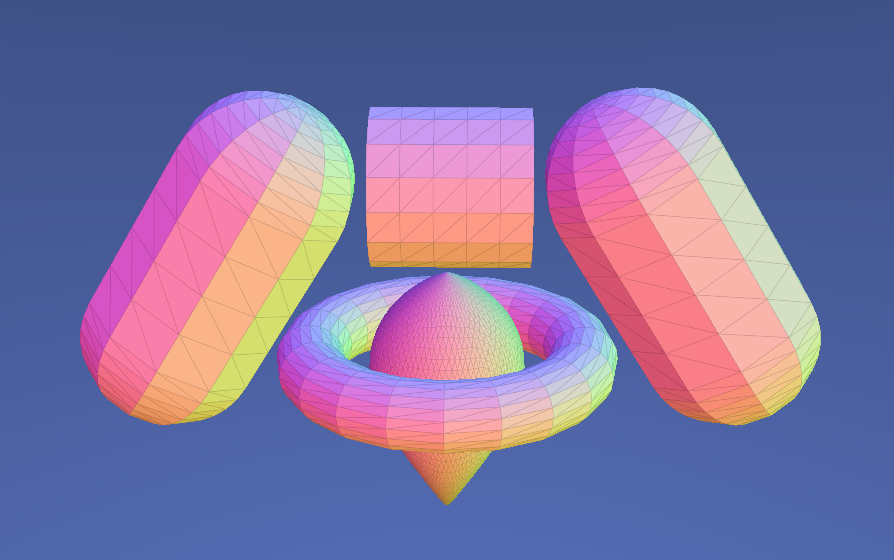
\includegraphics[width=0.75\textwidth]{Captures/transformations.png}}

	\caption{Union de maillages basiques. Les capsules ont été transformées par rotation et translation. L'icosphere au centre a été transformée par deux SphereWarp}
\end{figure}
\FloatBarrier
